\documentclass{article}

% packages
\usepackage{amsmath, amsthm, thmtools, amsfonts, amssymb, luacode, catchfile, tikzducks, hyperref, ifthen}
\ifcsname c@kobocompile\endcsname
	\usepackage[a5paper, total={1072pt, 1448pt}, margin=10pt, includeheadfoot]{geometry} % set page margins
\else
	\usepackage[a4paper, margin=50pt, includeheadfoot]{geometry}
\fi
\usepackage[shortlabels]{enumitem}
\usepackage[skip=3pt, indent=0pt]{parskip}

% language
\usepackage[bidi=basic, layout=tabular, provide=*]{babel}
\ifcsname c@english\endcsname
	\babelprovide[main, import]{english}
\else
	\babelprovide[main, import]{hebrew}
	\babelprovide{rl}
\fi
%\babelfont{rm}{Libertinus Serif}
\babelfont{rm}[Renderer=Harfbuzz]{Libertinus Serif}
\babelfont{sf}{Libertinus Sans}
\babelfont{tt}{Libertinus Mono}

% style
\AddToHook{cmd/section/before}{\clearpage}	% Add line break before section
\linespread{1.3}
\setcounter{secnumdepth}{0}		% Remove default number tags from sections, this won't do well with theorems
\AtBeginDocument{\setlength{\belowdisplayskip}{3pt}}
\AtBeginDocument{\setlength{\abovedisplayskip}{3pt}}
\graphicspath{ {../images/} }

% operators
\DeclareMathOperator\cis{cis}
\DeclareMathOperator\Sp{Sp}
\DeclareMathOperator\tr{tr}
\DeclareMathOperator\im{Im}
\DeclareMathOperator\re{Re}
\DeclareMathOperator\diag{diag}
\DeclareMathOperator*\lowlim{\underline{lim}}
\DeclareMathOperator*\uplim{\overline{lim}}
\DeclareMathOperator\rng{rng}
\DeclareMathOperator\Sym{Sym}
\DeclareMathOperator\Arg{Arg}
\DeclareMathOperator\Log{Log}
\DeclareMathOperator\dom{dom}
\DeclareMathOperator\supp{Supp}
\DeclareMathOperator\var{Var}
\DeclareMathOperator\cov{Cov}

% commands
%\renewcommand\qedsymbol{\textbf{מש''ל}}
%\renewcommand\qedsymbol{\fbox{\emoji{lizard}}}
\newcommand{\Aa}[0]{\mathcal{A}}
\newcommand{\Bb}[0]{\mathcal{B}}
\newcommand{\CC}[0]{\mathbb{C}}
\newcommand{\Cc}[0]{\mathcal{C}}
\newcommand{\EE}[0]{\mathbb{E}}
\newcommand{\FF}[0]{\mathbb{F}}
\newcommand{\Ff}[0]{\mathcal{F}}
\newcommand{\Ii}[0]{\mathcal{I}}
\newcommand{\Gg}[0]{\mathcal{G}}
\newcommand{\Ll}[0]{\mathcal{L}}
\newcommand{\Mm}[0]{\mathcal{M}}
\newcommand{\NN}[0]{\mathbb{N}}
\newcommand{\Nn}[0]{\mathcal{N}}
\newcommand{\PP}[0]{\mathbb{P}}
\newcommand{\Pp}[0]{\mathcal{P}}
\newcommand{\QQ}[0]{\mathbb{Q}}
\newcommand{\RR}[0]{\mathbb{R}}
\newcommand{\Rr}[0]{\mathcal{R}}
\newcommand{\Ss}[0]{\mathcal{S}}
\newcommand{\TT}[0]{\mathbb{T}}
\newcommand{\Uu}[0]{\mathcal{U}}
\newcommand{\Vv}[0]{\mathcal{V}}
\newcommand{\Ww}[0]{\mathcal{W}}
\newcommand{\ZZ}[0]{\mathbb{Z}}
\newcommand{\acts}[0]{\circlearrowright}
\newcommand{\explain}[2] {
	\begin{flalign*}
		 && \text{#2} && \text{#1}
	\end{flalign*}
}
\newcommand{\maketitleprint}[0]{ \begin{center}
	%\begin{tikzpicture}[scale=3]
	%	\duck[graduate=gray!20!black, tassel=red!70!black]
	%\end{tikzpicture}	
	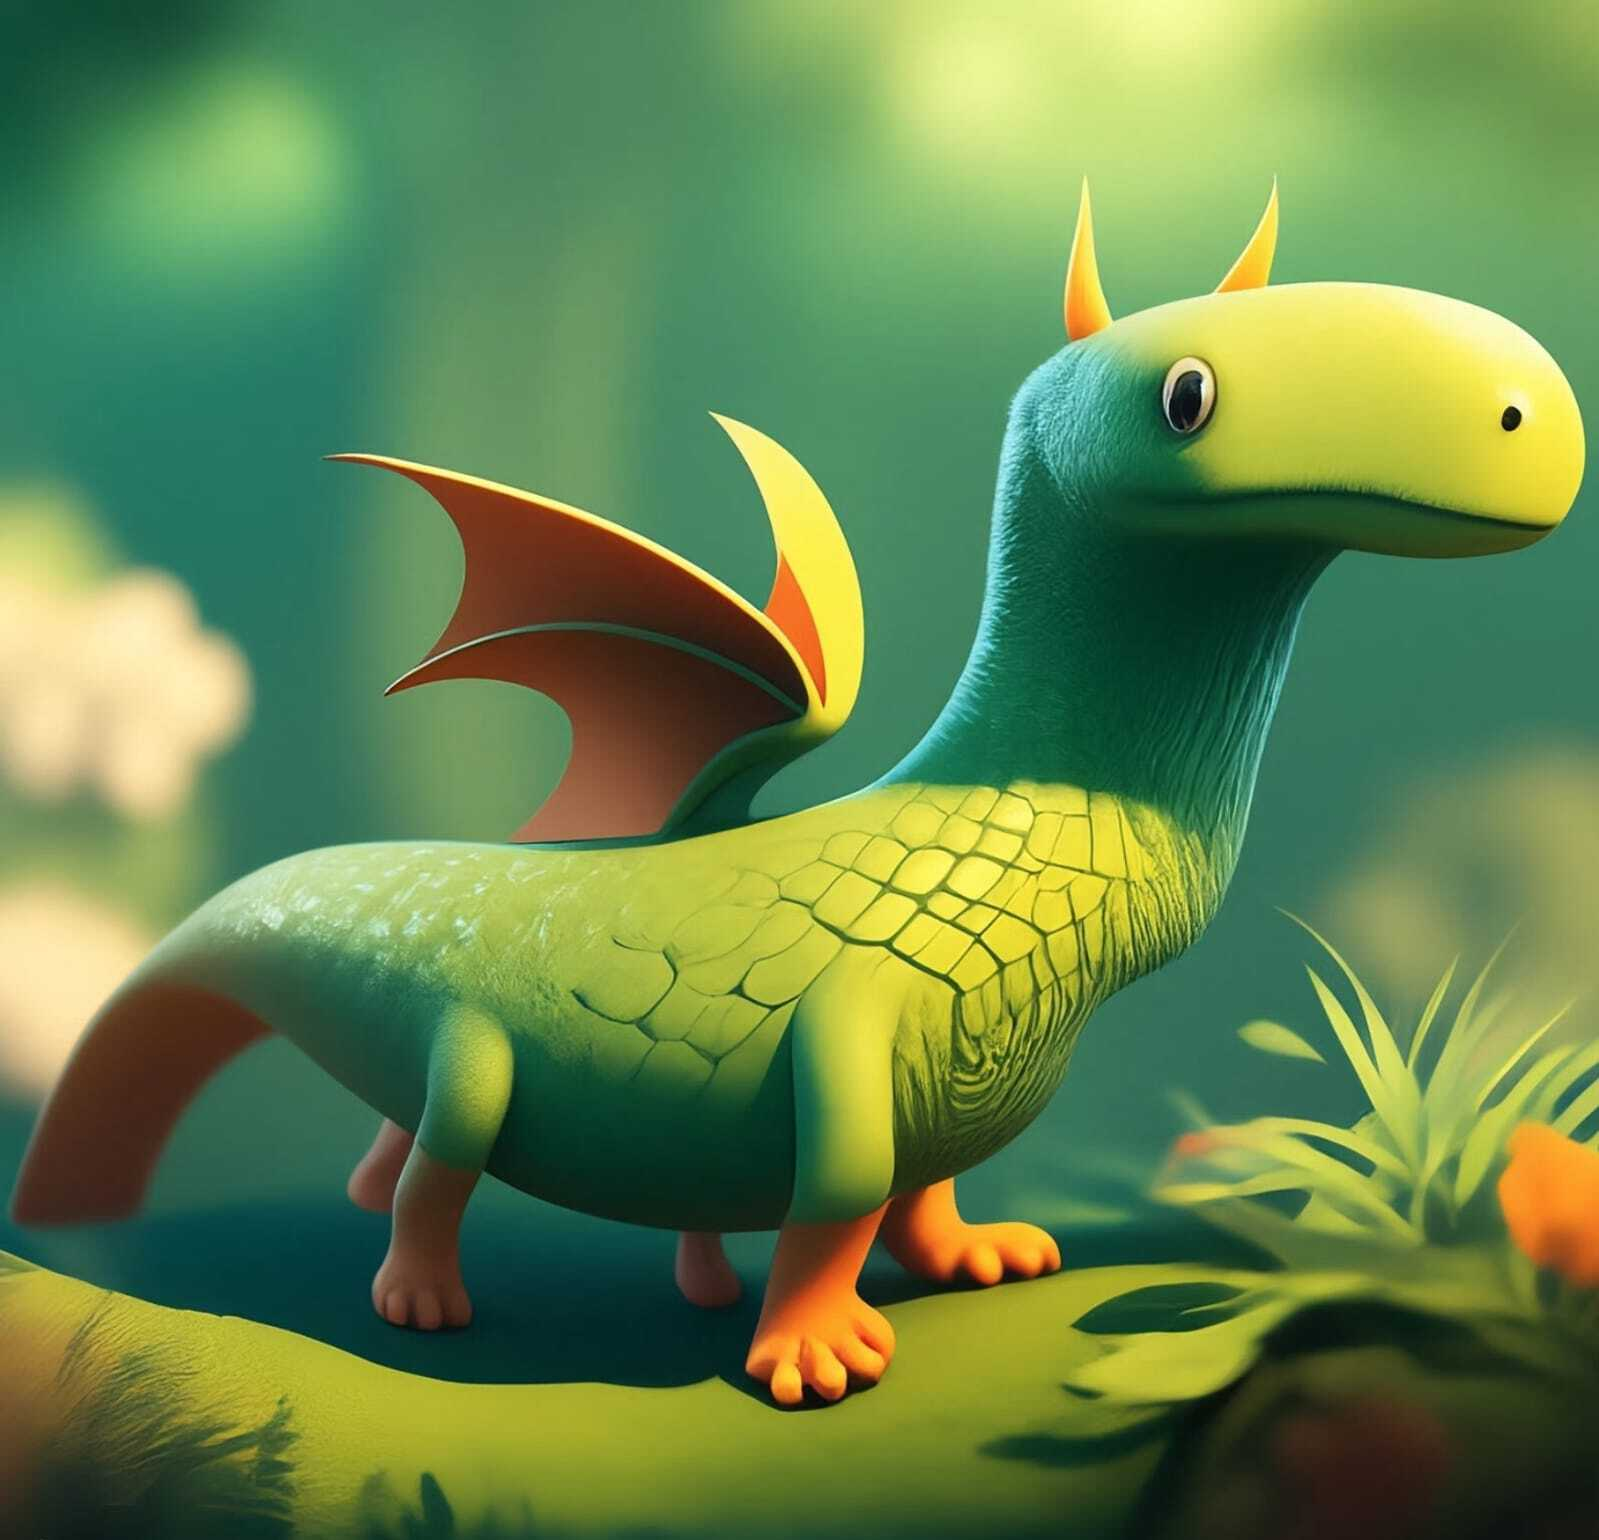
\includegraphics[width=6cm]{cover}
\end{center}
}

% theorem commands
\newtheoremstyle{c_remark}
	{}	% Space above
	{}	% Space below
	{}% Body font
	{}	% Indent amount
	{\bfseries}	% Theorem head font
	{}	% Punctuation after theorem head
	{.5em}	% Space after theorem head
	{\thmname{#1}\thmnumber{ #2}\thmnote{ \normalfont{\text{(#3)}}}}	% head content
\newtheoremstyle{c_definition}
	{3pt}	% Space above
	{3pt}	% Space below
	{}% Body font
	{}	% Indent amount
	{\bfseries}	% Theorem head font
	{}	% Punctuation after theorem head
	{.5em}	% Space after theorem head
	{\thmname{#1}\thmnumber{ #2}\thmnote{ \normalfont{\text{(#3)}}}}	% head content
\newtheoremstyle{c_plain}
	{3pt}	% Space above
	{3pt}	% Space below
	{\itshape}% Body font
	{}	% Indent amount
	{\bfseries}	% Theorem head font
	{}	% Punctuation after theorem head
	{.5em}	% Space after theorem head
	{\thmname{#1}\thmnumber{ #2}\thmnote{ \text{(#3)}}}	% head content

\ifcsname c@english\endcsname
	\theoremstyle{plain}
	\newtheorem{theorem}{Theorem}[section]
	\newtheorem{lemma}[theorem]{Lemma}
	\newtheorem{proposition}[theorem]{Proposition}
	\newtheorem*{proposition*}{Proposition}
	%\newtheorem{corollary}[theorem]{אין חלופה עברית}

	\theoremstyle{definition}
	\newtheorem{definition}[theorem]{Definition}
	\newtheorem*{definition*}{Definition}
	\newtheorem{example}{Example}[section]
	\newtheorem{exercise}{Exercise}[section]

	\theoremstyle{remark}
	\newtheorem*{remark}{Remark}
	\newtheorem*{solution}{Solution}
	\newtheorem{conclusion}[theorem]{Conclusion}
	\newtheorem{notation}[theorem]{Notation}
\else
	\theoremstyle{c_plain}
	\newtheorem{theorem}{משפט}[section]
	\newtheorem{lemma}[theorem]{למה}
	\newtheorem{proposition}[theorem]{טענה}
	\newtheorem*{proposition*}{טענה}
	%\newtheorem{corollary}[theorem]{אין חלופה עברית}

	\theoremstyle{c_definition}
	\newtheorem{definition}[theorem]{הגדרה}
	\newtheorem*{definition*}{הגדרה}
	\newtheorem{example}{דוגמה}[section]
	\newtheorem{exercise}{תרגיל}[section]

	\theoremstyle{c_remark}
	\newtheorem*{remark}{הערה}
	\newtheorem*{solution}{פתרון}
	\newtheorem{conclusion}[theorem]{מסקנה}
	\newtheorem{notation}[theorem]{סימון}
\fi

% Questions related commands
\newcounter{question}
\setcounter{question}{1}
\newcounter{sub_question}
\setcounter{sub_question}{1}

\ifcsname c@english\endcsname
	\newcommand{\question}[1][0]{
		\ifthenelse{#1 = 0}{}{\setcounter{question}{#1}}
		\section{Question \arabic{question}}
		\addtocounter{question}{1}
		\setcounter{sub_question}{1}
	}

	\newcommand{\subquestion}[1][0]{
		\ifthenelse{#1 = 0}{}{\setcounter{sub_question}{#1}}
		\subsection{Part \alph{sub_question}}
		\addtocounter{sub_question}{1}
	}
\else
	\newcommand{\question}[1][0]{
		\ifthenelse{#1 = 0}{}{\setcounter{question}{#1}}
		\section{שאלה \arabic{question}}
		\addtocounter{question}{1}
		\setcounter{sub_question}{1}
	}

	\newcommand{\subquestion}[1][0]{
		\ifthenelse{#1 = 0}{}{\setcounter{sub_question}{#1}}
		\subsection{סעיף \localecounter{letters.gershayim}{sub_question}}
		\addtocounter{sub_question}{1}
	}
\fi

% import lua and start of document
\directlua{common = require ('../common')}

\GetEnv{AUTHOR}

% headers
\author{\AUTHOR}
\date\today

\title{פתרון מטלה מסכמת --- אנליזה על יריעות, 80426}
% chktex-file 17
% chktex-file 9

\DeclareMathOperator{\vol}{vol}
\DeclareMathOperator{\Div}{div}
\DeclareMathOperator{\curl}{curl}

\begin{document}
\maketitle
\maketitleprint[blue]

\question{}
נתאר את הוכחת משפט הדיברגנץ ליריעות קומפקטיות עם שפה.
\begin{proof}
	בגרסה ללא השפה האסטרטגיה הייתה בנייה של זרימה מתאימה לשדה הווקטורי הנתון $X$ על־ידי שימוש בזרימה מקומית וקומפקטיות.
	לבסוף על־ידי שימוש במשפט הווריאציה הראשונה נוכל לקבל שקילות לאינטגרל על הדיברגנץ, היא מקבעת את ערכו לאפס.

	עתה נתאר את משפט הדיברגנץ עצמו, ניסוח המשפט הוא חלק משמעותי בהוכחתו, והוא נכתב כעת מתוך התפיסה שיש לזכור אותו בדיוק.
	תהי $M^k \subseteq \RR^n$ יריעה קומפקטית עם שפה.
	נניח גם ש־$X : M \to \RR^n$ שדה וקטורי משיק ל־$M$, כלומר ש־$X(p) \in T_p(M)$ לכל $p \in M$.
	אז מתקיים,
	\[
		\int_M \Div_M X\ d\vol_k
		= \int_{\partial M} \langle X(p), \nu(p) \rangle\ d\vol_{k - 1}(p)
	\]
	כלומר ערך האינטגרל הוא ערך האינטגרל בשפה של מכפלה בנורמל חיצוני, שלא במפתיע אין תלות בפנים (ולמעשה כבר עתה יכולנו להוכיח זאת ישירות עם אדיטיביות האינטגרל וחלוקה לשפה ופנים), והתלות היא בכמה היריעה התרחבה עם $X$.

	לאחר הבנה מעמיקה של המשפט, נוכל להסביר את הוכחתו, היא כיאה לכל משפט מרכזי באנליזה מתחילה ברדוקציות.
	הרדוקציה שאנו נעשה היא זו שתאפשר לנו להניח שהשדה הווקטורי $X$ הוא מכווץ בלבד, ובכך נוכל להשתמש באסטרטגיה שנראה בהמשך.
	פורמלית נוכיח כי,
	\[
		\langle X(p), \nu(p) \rangle < 0
	\]
	ונוכל להשיג אותו על־ידי שימוש בקומפקטיות ובמציאת מקסימום של $X$ על השפה $\partial M$, נוכל לבנות יריעה חדשה שמזיזה את $X$ פנימה בלבד, ונעשה זאת ככה שנוכל לחשב את האינטגרל בקלות ובהתאם לקבל את הרדוקציה.

	עתה נגיע לחלק הבא, שלב הבניות.
	המטרה שלנו היא לפרק את $M$ בדרך הנוחה ביותר, ונעשה זאת על־ידי הגדרת ''משיכת שפה'', כלומר נגדיר את הזרימה החד־צדדית שמובטח לנו שקיימת, ונגדיר את היריעה $N_t = \varphi([0, t] \times \partial M)$.
	המפתח בשלב זה עבורי הוא תפיסה טובה של משמעות $N_t$, וכאמור ניתן לתאר אותו כמשיכה ש־$\varphi$ מבצעת על השפה, נוכל לדמיין זאת על־ידי סימון השפה ביריעה, הפעלת $\varphi$ ובדיקת המיקומים שהשפה עוברת בהם.
	מבנה זה מאפשר לנו לבצע את הפירוק (עד כדי חיתוך ממידה אפס),
	\[
		M = \varphi_t(M) \cup N_t
	\]
	ובהתאם לטענה האחרונה, נוכל גם להסיק,
	\[
		\vol_k(M)
		= \vol_k(\varphi_t(M)) + \vol_k(N_t)
	\]
	אם נגזור את הביטוי נקבל אם כך,
	\[
		0 = 
		\left. \frac{d}{dt} \vol_k(\varphi_t(M)) \right\lvert_{t = 0}
		+ \left. \frac{d}{dt} \vol_k(N_t) \right\lvert_{t = 0}
	\]
	ועל־ידי שימוש שקול לגרסה ללא שפה במשפט הווריאציה הראשונה גם,
	\[
		\int_M \Div_M(X)\ d\vol_k
		= - \left. \frac{d}{dt} \vol_k(N_t) \right\lvert_{t = 0}
	\]
	כלומר עלינו לנתח את $N_t$ בלבד כדי למצוא את הטענה.
	אבל ישירות מהגדרת $N_t$ אנו יודעים כי (על־ידי שימוש בפוביני),
	\[
		\vol_k(N_t)
		= \int_{\partial M} \int_{0}^{t} V(D \varphi |_{(x, s)})\ ds\ d\vol_{k - 1}(x)
	\]
	מהמשפט היסודי של החשבון האינפיניטסימלי נוכל להסיק שגם,
	\[
		- \frac{d}{dt} \left. \vol_k(N_t) \right\lvert_{t = 0}
		= \int_{\partial M} V(D \varphi |_{(x, 0)})\ d\vol_{k - 1}(x)
	\]
	כלומר המשפט כולו שקול לטענה שמתקיים,
	\[
		V(D \varphi |_{(x, 0)}) = - \langle X(x), \nu(x) \rangle
	\]
	טענה זו נובעת משימוש בהוכחה סטנדרטית של בחירת בסיס ושימוש באפיון השקול של אופרטור נפח וברדוקציה הראשונה.
\end{proof}
הוכחה זו כתובה כך שהחלקים שניתנים להשלמה עבורי הושמטו, כל מה שנכתב הוא מה שהייתי כותב גם במפתח הוכחה עבור שינונה לקראת מבחן.

\question{}
\subquestion{}
נוכיח את משפט הפונקציה ההפוכה לנקודות שפה. \\
תהינה $M \subseteq \RR^m, N \subseteq \RR^n$ יריעות עם שפה.
נניח גם ש־$f : M \to N$ העתקה חלקה כך ש־$f(\partial M) \subseteq \partial N$.
נסמן $p \in \partial M$ ו־$q \in \partial N$ נקודות כך ש־$f(p) = q$ ו־$D f |_p : T_p M \to T_q N$ איזומורפיזם לינארי. \\
נראה שקיימות סביבות פתוחות $p \in U \subseteq M$ ו־$q \in V \subseteq N$ כך ש־$f |_U : U \to V$ היא דיפאומורפיזם.
\begin{proof}
	נסמן $k = \dim M$.
	תהי $\alpha : W_0 \to M$ פרמטריזציה מקומית כך ש־ $W_0 \subseteq \HH^k$, ראינו כי אם נקודה שייכת לשפה אז הפרמטריזציה של השפה של $\HH^k$ הולכת לשפה של היריעה, וכן $0 \in \partial \HH^k$ נניח בלי הגבלת הכלליות ש־$\alpha(0) = p$.
	נסמן גם $\beta : \Omega_0 \to N$ פרמטריזציה מקומית סביב $q$, גם הפעם נניח $\Omega_0 \subseteq \HH^k, \beta(0) = q$.
	נגדיר את הפונקציה $g : U_0 \to \HH^k$ עבור $U_0 \subseteq \HH^k$ על־ידי,
	\[
		g = \beta^{-1} \circ f \circ \alpha
	\]
	כאשר $U_0$ הוא סביבה פתוחה (בטופולוגיה המושרית) אשר ידוע שקיימת מבחירת סביבה קטנה מספיק.
	מההנחה שלנו מתקיים $g(0) = 0$ וכן,
	\[
		\forall x \in \partial \HH^k,\ 
		g(x) \in \partial \HH^k
	\]
	לבסוף גם נבחין כי $0$ נקודה רגולרית של $g$, הסיבה היא שנתון ש־$f$ רגולרית בנקודה זו במובן של מרחבים מטריים, וכן פרמטריזציות הן הפיכות מקומית.
	לכן מספיק להוכיח את הטענה עבור מקרה זה, כלומר ביצענו תרגום של הבעיה לבעיה במרחבים מטריים.

	נבנה פונקציה חדשה המבוססת על $g$,
	\[
		h(x)
		= \begin{cases}
			g(x) & x_k \ge 0 \\
			- g(-x) & x_k < 0
		\end{cases}
	\]
	משימוש בכלל השרשרת נקבל ש־$h$ היא פונקציה דיפרנציאבילית בכל נקודה ב־$U_1 = U_0 \cup \{ -x | x \in U_0 \}$, ובפרט היא דיפרנציאבילית ב־$x = 0$ ומתקיים,
	\[
		D h |_0
		= D g |_0
	\]
	נבחין כי בבנייה זו השתמשנו בעובדה ש־$\forall x \in \partial U_0,\ g(x) \in \partial \HH^k$ וכן בעובדה החשובה לא פחות ש־$\forall x \in U_0^\circ,\ g(x) \in {(\HH^k)}^\circ$.
	אבל נתון כי $D g |_0$ רגולרית ולכן גם $D h |_0$ רגולרית וקיימת סביבה פתוחה בה $h$ מוגדרת סביב $0$, לכן משפט הפונקציה ההפוכה חל וקיימת סביבה $U_2 \subseteq U_1$ כך ש־$h |_{U_2} : U_2 \to U_2$ הפיכה ולכן גם דיפאומורפיזם חלק.
	לבסוף נגדיר $U = U_2 \cap U_0$ ונקבל ש־$g \restriction U = h \restriction U$ ולכן $g$ דיפאומורפיזם חלק תחת הצמצום.
\end{proof}

\subquestion{}
נניח ש־$M^k \subseteq \RR^n$ יריעה ללא שפה,
ותהי $U \subseteq \RR^k$ פתוחה כלשהי.
נניח ש־$\alpha : U \to M$ היא חלקה כך ש־$D \alpha |_x$ מדרגה $k$ לכל $x \in U$. \\
נראה ש־$\alpha$ היא העתקה פתוחה.
\begin{proof}
	עבור נקודה כלשהי $x \in U$ מהנתון $\alpha$ רגולרית ב־$x$ ולכן ממשפט הפונקציה ההפוכה $\alpha |_V : V \to \alpha(V)$ היא דיפאומורפיזם הפיך, כאשר $x \in V \subseteq U$ פתוחה.
	אבל טענה זו נכונה לכל $x$, כלומר $\alpha$ הפיכה מקומית בכל מקום, ולכן הפיכה ובהתאם גם דיפאומורפיזם ולכן בפרט הומיאומורפיזם ומאפיון שקול העתקה פתוחה.
\end{proof}

\subquestion{}
בהגדרה של יריעות פתוחות פרמטריזציה דורשת את תנאי הפתיחות, אבל בסעיף הקודם מצאנו שפתיחות נובעת מקיום העתקה חלקה לסביבה של היריעה.
אנו נסביר עתה את הקשר שבין שתי הטענות הלכאורה מעט סותרות הללו.
\begin{solution}
	בהוכחת הטענה כבר התבססנו על תכונת הפתיחות המקומית של היריעה, למעשה הטענה שראינו בסעיף ב' היא דרך מצוינת להבין מה היא יריעה.
	כלומר, נוכל להסיק שיריעה מתנהגת באופן מספיק ''יפה'' כדי לאפשר לפונקציות רגולריות להיות גם פתוחות באופן ישיר, ובכך הן האובייקט שקושר בין דיפאומורפיזם (ובפרט הומיאומורפיזם ופתיחות) לבין קבוצה במרחב.
\end{solution}

\question{}
נסמן ב־$C$ את מעגל היחידה במישור $xy$ ב־$\RR^3$, כלומר $C = \partial \{ (x, y, 0) \in \RR^3 \mid x^2 + y^2 = 1 \}$,
ונסמן גם את הפרמטריזציה שלו,
\[
	\gamma(t)
	= (\cos t, \sin t, 0)
\]
נגדיר את השדה הווקטורי $F$ על $\RR^3 \setminus C$ המוגדר על־ידי,
\[
	F(x)
	= \int_{0}^{2 \pi} \frac{x - \gamma(t)}{{\lVert x - \gamma(t) \rVert}^3} \times \gamma'(t)\ dt
\]
כאשר,
\[
	{(u_1, u_2, u_3)}^t \times {(v_1, v_2, v_3)}^t
	= {(u_2 v_3 - u_3 v_2, u_3 v_1 - u_1 v_3, u_1 v_2 - u_2 v_1)}^t
\]
וכאשר האינטגרל מבוצע קורדינטה־קורדינטה.

\subquestion{}
נראה ש־$F$ הוא משמר מקומית.
\begin{proof}
	ניזכר כי $F$ משמר מקומית אם ורק אם,
	\[
		\frac{\partial F_i}{\partial x_j}
		= \frac{\partial F_j}{\partial x_i}
	\]
	לכל $i, j \in [3]$. \\
	תהי $p \in \RR^3$, נגדיר ${\{ e_i \}}_{i = 1}^3 \subseteq \RR^3$ הבסיס הסטנדרטי של המרחב, ונחשב,
	\begin{align*}
		\nabla {\lVert x - p \rVert}^{-1}
		& = \nabla {\left(\sum_{i = 1}^3 {(x_i - p_i)}^2 \right)}^{-1/2} \\
		& = \sum_{j = 1}^3 - \frac{1}{2} \cdot 2 (x_j - p_j) \cdot {\left(\sum_{i = 1}^3 {(x_i - p_i)}^2 \right)}^{-3/2} e_j \\
		& = \sum_{j = 1}^3 \frac{p_j - x_j}{{\lVert x - p \rVert}^3} e_j \\
		& = \frac{p - x}{{\lVert x - p \rVert}^3}
	\end{align*}
	לכן אם נסמן $\phi(x) = \frac{1}{\lVert x \rVert}$ אז,
	\[
		F(x)
		= \int_{0}^{2 \pi} \nabla \phi(x - \gamma(t)) \times \gamma'(t)\ dt
	\]
	נבחין כי $\nabla \phi(x) = \frac{x}{{\lVert x \rVert}^3}$ ונחשב את הלפלסיאן,
	\[
		\frac{\partial}{\partial x_1} \phi(x)
		= \frac{x_1}{{\lVert x \rVert}^3}
		\implies
		\frac{\partial^2}{\partial x_1^2} \phi(x)
		= \frac{{\lVert x \rVert}^3 - 3 x_1^2 \lVert x \rVert}{{\lVert x \rVert}^6}
	\]
	ולכן נובע,
	\[
		\Delta \phi
		= \frac{\partial}{\partial x_1} \phi + \frac{\partial}{\partial x_2} \phi + \frac{\partial}{\partial x_3} \phi
		= \frac{3 {\lVert x \rVert}^3 - 3 (x_1^2 + x_2^2 + x_3^2) \lVert x \rVert}{{\lVert x \rVert}^6}
		= 0
	\]

	עתה נחשב,
	\begin{align*}
		\frac{\partial F_3}{\partial x_2} - \frac{\partial F_2}{\partial x_3}
		& = \partial_2 \int_{0}^{2 \pi} (\partial_1 \phi(x - \gamma(t)) \cos t + \partial_2 \phi(x - \gamma(t)) \sin t)\ dt - \partial_3 \int_{0}^{2 \pi} (- \partial_3 \phi(x - \gamma(t)) \sin t)\ dt \\
		& = \int_{0}^{2 \pi} \partial_2 (\partial_1 \phi(x - \gamma(t)) \cos t + \partial_2 \phi(x - \gamma(t)) \sin t) + \partial_3 (\partial_3 \phi(x - \gamma(t)) \sin t)\ dt \\
		& = \int_{0}^{2 \pi} \partial_2 \partial_1 \phi(x - \gamma(t)) \cos t + \partial_2^2 \phi(x - \gamma(t)) \sin t + \partial_3^2 \phi(x - \gamma(t)) \sin t\ dt \\
		& = \int_{0}^{2 \pi} \partial_1 \partial_2 \phi(x - \gamma(t)) \cos t - \partial_1^2 \phi(x - \gamma(t)) \sin t\ dt \\
		& = \partial_1 \int_{0}^{2 \pi} \partial_2 \phi(x - \gamma(t)) \cos t - \partial_1 \phi(x - \gamma(t)) \sin t\ dt \\
		& = \partial_1 \int_{0}^{2 \pi} \frac{(x_2 - \sin t) \cos t - (x_1 - \cos t) \sin t}{{\lVert x - \gamma(t) \rVert}^3}\ dt \\
		& = \partial_1 \int_{0}^{2 \pi} \frac{\langle x, \gamma'(t) \rangle}{{\lVert x - \gamma(t) \rVert}^3}\ dt
	\end{align*}
	אבל זהו אינו אלא אינטגרל מסילתי, כלומר,
	\[
		\frac{\partial F_3}{\partial x_2} - \frac{\partial F_2}{\partial x_3}
		= \partial_1 \int_{S^1} \nabla \phi(x)\ dl
		= 0
	\]
	ישירות משימוש בפוטנציאל באינטגרציה.
	נוכל להסיק באותו תהליך בדיוק שגם,
	\[
		\frac{\partial F_1}{\partial x_2} - \frac{\partial F_2}{\partial x_1}
		= \partial_3 \int_{S^1} \nabla \phi(x)\ dl
		= 0
	\]
	וכן,
	\[
		\frac{\partial F_1}{\partial x_3} - \frac{\partial F_3}{\partial x_1}
		= \partial_2 \int_{S^1} \nabla \phi(x)\ dl
		= 0
	\]
	לכן מהגדרת שימור מקומי נסיק ש־$F$ משמר מקומית ב־$\RR^3 \setminus C$.
\end{proof}

\subquestion{}
נגדיר את המסילה $\mu = \mu_R : [-R, R] \to \RR^3 \setminus C$ על־ידי,
\[
	\mu(t)
	= (0, 0, t)
\]
ונחשב את האינטגרל המסילתי,
\[
	I = \int_{\mu} F\ dl
\]
\begin{solution}
	מהגדרה,
	\[
		I
		= \int_{-R}^{R} F(\mu(t)) \cdot \mu'(t)\ dt
		= \int_{-R}^{R} F(0, 0, t) \cdot (0, 0, 1)\ dt
		= \int_{-R}^{R} F_3(0, 0, t)\ dt
	\]
	אבל ישירות מהגדרת מכפלה וקטורית,
	\begin{align*}
		F_3(0, 0, t)
		& = \int_{0}^{2 \pi} \frac{0 - \cos u}{{\lVert (0, 0, t) - \gamma(u) \rVert}^3} \cdot (\cos u) - \frac{0 - \sin u}{{\lVert (0, 0, t) - \gamma(u) \rVert}^3} \cdot (- \sin u)\ du \\
		& = - \int_{0}^{2 \pi} \frac{\sin^2 u + \cos^2 u}{{(\cos^2 u + \sin^2 u + t^2)}^{3 / 2}}\ du \\
		& = - \int_{0}^{2 \pi} \frac{1}{{(1 + t^2)}^{3 / 2}}\ du \\
		& = \frac{-2 \pi}{{(1 + t^2)}^{3 / 2}}
	\end{align*}
	ולכן בהצבה נקבל,
	\[
		I
		= \int_{-R}^{R} F_3(0, 0, t)\ dt
		= \int_{-R}^{R} \frac{-2 \pi}{{(1 + t^2)}^{3 / 2}}\ dt
		= - 2 \pi {\left[ \frac{t}{\sqrt{1 + t^2}}\right]}_{t = -R}^{t = R}
		= - 2 \pi \left(\frac{R}{\sqrt{1 + R^2}} - \frac{-R}{\sqrt{1 + R^2}}\right)
		= \frac{-4 \pi R}{\sqrt{1 + R^2}}
	\]
\end{solution}

\subquestion{}
נגדיר את המשטח,
\[
	Q_R
	= [(0, 0, -R), (0, 0, R)] + [(0, 0, R), (2R, 0, R)] + [(2R, 0, R), (2R, 0, -R)] + [(2R, 0, -R), (0, 0, -R)]
\]
ונסמן את המקטעים $\mu_1, \mu_2, \mu_3, \mu_4$. \\
נחשב את,
\[
	L_{\infty}
	= \lim_{R \to \infty} \int_{Q_R} F\ dl
\]
\begin{solution}
	על־ידי שימוש בזהויות מוכרות ובאי־השוויון הנתון $\lVert u \times v \rVert \le \lVert u \rVert \cdot \lVert v \rVert$ נסיק,
	\begin{align*}
		\left\lVert \int_{\mu_2} F(t)\ dt \right\rVert
		& \le \int_{\mu_2} \left\lVert F(p) \right\rVert\ dl \\
		& \le \int_{\mu_2} \int_{0}^{2 \pi} \frac{\lVert p - \gamma(t) \rVert}{{\lVert p - \gamma(t) \rVert}^3} \cdot \lVert \gamma'(t) \rVert\ dt\ dl \\
		& = \int_{\mu_2} \int_{0}^{2 \pi} \frac{dt\ dl}{{\lVert p - \gamma(t) \rVert}^2} \\
		& = \int_{0}^{2R} \int_{0}^{2 \pi} \frac{|\mu_2'(u)| \cdot dt\ du}{{\lVert \mu_2(u) - \gamma(t) \rVert}^2} \\
		& = \int_{-R}^{R} \int_{0}^{2 \pi} \frac{dt\ du}{{(\cos t - u)}^2 + \sin^2 t + R^2} \\
		& = \int_{-R}^{R} \int_{0}^{2 \pi} \frac{dt\ du}{u^2 + 2u \cos t + 1 + R^2} \\
		& \le \int_{-R}^{R} \int_{0}^{2 \pi} \frac{dt\ du}{u^2 + 1 + R^2} \\
		& = \int_{-R}^{R} \frac{2 \pi\ du}{u^2 + 1 + R^2} \\
		& \xrightarrow{R \to \infty} 0
	\end{align*}
	באופן שקול נוכל לקבל שאיפה לאפס של $\int_{\mu_4} F(t)\ dt$, ולכן נותר לנו לחשב את האינטגרל המסילתי על $\mu_3$.
	\begin{align*}
		\int_{\mu_3} F(t)\ dt
		& = \int_{\mu_3} \int_{0}^{2 \pi} \frac{0 - \cos u}{{\lVert (2R, 0, t) - \gamma(u) \rVert}^3} \cdot (\cos u) - \frac{2R - \sin u}{{\lVert (2R, 0, t) - \gamma(u) \rVert}^3} \cdot (- \sin u)\ du\ dt \\
		& = \int_{\mu_3} \int_{0}^{2 \pi} \frac{- \cos^2(u) - \sin^2(u) + 2R \sin t}{{\lVert {(2R - \cos u)}^2 + \sin^2(u) + t^2 \rVert}^3}\ du\ dt \\
		& = \int_{-R}^{R} \int_{0}^{2 \pi} \frac{-1 + 2R \sin t}{\lvert {4R^2 - 4 \cos u + 1 + t^2 \rvert}^{3 / 2}}\ du\ dt \\
		& \xrightarrow{R \to \infty} 0
	\end{align*}
	משיקולי חסימה על־ידי אינטגרל מהצורה של הסעיף הקודם.
	נסיק אם כן ש־$L_{\infty} = \lim_{R \to \infty} \frac{-4 \pi R}{\sqrt{1 + R^2}} = -4 \pi$ בלבד.
\end{solution}

\subquestion{}
נראה ש־$\int_{Q_1} F\ dl = L_{\infty}$ ונסיק ש־$F$ לא משמרת ובהתאם ש־$\RR^3 \setminus C$ לא פשוטת קשר.
\begin{proof}
	נגדיר $T_R \overset{\operatorname{def}}{=} Q_R \setminus {\{ 0 \}}^2 \times [-1, 1]$, אז $T_{R_1}$ שקול הומוטופית מסילתית ל־$T_{R_2}$ לכל $R_1, R_2 > \frac{1}{2}$, אבל $F$ שדה משמר מקומית ולכן האינטגרלים שלהם שווים.
	אז נסיק,
	\[
		\int_{T_1} F\ dl
		= \int_{T_R} F\ dl
		\xrightarrow{R \to \infty} L_{\infty} - I
	\]
	עבור,
	\[
		I = \int_{Q_1} F\ dl
		= \int_{\mu_1} F\ dl
		= \frac{-4 \pi \cdot 1}{\sqrt{1 + 1^2}}
		= - 2 \sqrt{2} \pi
	\]
	כלומר מצאנו שבדיוק מתקיים $\int_{Q_1} F\ dl = L_{\infty}$.

	אילו הייתה $\RR^3 \setminus C$ פשוטת קשר, אז ערך כל אינטגרל מסילתי על לולאה היה $0$, לכן ערך אינטגרל זה (שאיננו מתאפס) מהווה סתירה ישירה להנחה כי התחום פשוט קשר.
	למעשה ידענו זאת כבר כי החבורה היסודית שלו היא $\ZZ \ne \{ 1 \}$.
\end{proof}

\question{}
תהינה $M^k \subseteq \RR^m, N^k \subseteq \RR^n$ שתי יריעות. \\
נגדיר את הדיפאומורפיזם החלק $F : M \to N$ כאיזומטריה אם לכל $p \in M$ ולכל $v, w \in T_p M$ מתקיים,
\[
	\langle v, w \rangle
	= \langle d F |_p (v), d F |_p (w) \rangle
\]
כלומר ש־$DF |_p : T_p M \to T_{F(p)} N$ היא איזומטריה.

\subquestion{}
נראה שאם $F : M \to N$ איזומטריה וכן $M, N$ שתיהן קומפקטיות, \\
אז $\vol_k(M) = \vol_k(N)$ וכן לכל מסילה חלקה $\gamma : [a, b] \to M$ מתקיים $L(\gamma) = L(F \circ \gamma)$.
\begin{proof}
	נניח ש־$p \in M$ וכן ש־$p \in U \subseteq M$ סביבה פתוחה כך ש־$\alpha : W \to U$ פרמטריזציה מקומית, ו־$W \subseteq \HH^k$.
	אז $\beta = F \circ \alpha$ פרמטריזציה מקומית של $q = F(p) \in N$.
	נסמן,
	\[
		T_x = D \alpha |_x,
		\quad
		S_x
		= D \beta |_x
		= (D F |_{\alpha(x)}) \circ D \alpha |_x
		= (D F |_{\alpha(x)}) \circ T_x
	\]
	אז מתקיים,
	\begin{align*}
		V(T_x)
		& = \sqrt{\det\left({(\langle T_x(e_i), T_x(e_j) \rangle)}_{i, j \in [k]}\right)} \\
		& = \sqrt{\det\left({(\langle D F |_x T_x(e_i), D F |_x T(e_j) \rangle)}_{i, j \in [k]}\right)} \\
		& = \sqrt{\det\left({(\langle S_x(e_i), S_x(e_j) \rangle)}_{i, j \in [k]}\right)} \\
		& = V(S_x)
	\end{align*}
	ולכן נובע,
	\[
		\int_U 1\ d\vol_k
		= \int_{W} 1\ V(T_x)\ dx
		= \int_{W} 1\ V(S_x)\ dx
		\int_{F(U)} 1\ d\vol_k
	\]
	ומכאן תוך שימוש בהגדרת היריעה (הגדרת חלוקת יחידה ושימוש חזור בטענה שעתה הוכחנו) נקבל שהנפחים זהים.

	נניח ש־$\gamma : [a, b] \to M$, אז,
	\[
		L(\gamma)
		= \int_{a}^{b} \lVert \gamma'(t) \rVert\ dt
		= \int_{a}^{b} \langle \gamma'(t), \gamma'(t) \rangle\ dt
		= \int_{a}^{b} \langle D F |_t \gamma'(t), D F |_t \gamma'(t) \rangle\ dt
		= \int_{a}^{b} \lVert (F \circ \gamma)'(t) \rVert\ dt
		= L(F \circ \gamma)
	\]
	ומצאנו כי השוויון מתקיים אף הוא.
\end{proof}

\subquestion{}
נניח ש־$F : S^n(1) \to S^n(2)$ הדיפאומורפיזם החלק בין ספירה ברדיוס $1$ לספירה ברדיוס $2$ ב־$\RR^{n + 1}$, כאשר $F(x) = 2x$.
נוכיח כי $F$ היא לא איזומטריה.
\begin{proof}
	נניח בשלילה שהיא איזומטריה ולכן בפרט המסילה $\gamma : [0, 1] \to \{ (\cos t, \sin t) \} \times {\{ 0 \}}^{n - 1}$ מקיימת,
	\[
		2 \pi
		= L(\gamma)
		= L(F \circ \gamma)
		= 2 \pi \cdot 2
	\]
	וזו סתירה.
\end{proof}

\subquestion{}
תהינה היריעות,
\[
	M = (0, 2 \pi) \times (0, 1) \subseteq \RR^2,
	\quad
	N = \{ (x, y) \in \RR^2 \mid x^2 + y^2 = 1, (x, y) \ne (1, 0) \} \times (0, 1) \subseteq \RR^3
\]
שתי היריעות הנתונות הן איזומטריות, אנו נמצא איזומטריה $F : M \to N$ ונסביר על שימושיה.
\begin{solution}
	נגדיר,
	\[
		F(t, y)
		= (\cos t, \sin t, y)
	\]
	ונראה שזו אכן איזומטריה.
	נתחיל להראות שהיא דיפאומורפיזם חלק.
	היא מוגדרת היטב כהרכבת פונקציות, היא חד־חד ערכית מחד־חד ערכיות של $(\cos t, \sin t) \simeq e^{it}$ וכי בקורדינטה השלישית היא הזהות, והיא על על־ידי בחירה של $(\Arg (x, y), t)$.
	היא חלקה כהרכבת פונקציות חלקות, ולכן מהווה דיפאומורפיזם חלק.

	נסמן $p = (t, y)$.
	מחישוב עולה כי,
	\[
		D F |_p
		= \begin{pmatrix}
			- \sin t & 0 \\
			\cos t & 0 \\
			0 & 1
		\end{pmatrix} 
	\]
	ואם $v = (v_1, v_2), w = (w_1, w_2)$ אז,
	\[
		D F |_{p}(v)
		= \begin{pmatrix} - v_1 \sin t \\ v_1 \cos t \\ v_2 \end{pmatrix},
		\quad
		D F |_{p}(w)
		= \begin{pmatrix} - w_1 \sin t \\ w_1 \cos t \\ w_2 \end{pmatrix}
	\]
	לבסוף נציב,
	\[
		\langle D F |_p(u), D F |_p(w) \rangle
		= v_1 w_1 \sin^2 t + v_1 w_1 \cos^2 t + v_2 w_2
		= v_1 w_1 + v_2 w_2
		= \langle v, w \rangle
	\]
	ומצאנו כי מתקיימת ההגדרה לאיזומטריה.

	לפעמים אני לוקח דף ומגלגל אותו לטלסקופ, המרחקים על הדף לא משתנים, אבל הדף משנה את צורתו מ־$M$ ל־$N$.
\end{solution}

\subquestion{}
נניח ש־$U \subseteq \RR^2$ קבוצה פתוחה, ונניח ש־$M \subseteq \RR^3$ יריעה איזומטרית ל־$U$. \\
נסמן $\alpha : U \to M$ האיזומטריה ביניהן, ונראה שאם $\alpha(x_0, y_0) = p$ ואם,
\[
	B = 
	\left\{
	\left. \frac{\partial^2 \alpha}{\partial x \partial y} \right\rvert_{(x_0, y_0)},
	\left. \frac{\partial^2 \alpha}{\partial^2 x} \right\rvert_{(x_0, y_0)},
	\left. \frac{\partial^2 \alpha}{\partial^2 y} \right\rvert_{(x_0, y_0)}
	\right\}
\]
אז $T_p M \perp B$.
\begin{proof}
	נחשב,
	\begin{align*}
		0
		& \overset{(1)}{=}  \frac{\partial}{\partial y} \left\langle (1, 0), (1, 0) \right\rangle \\
		& \overset{(2)}{=}  \frac{\partial}{\partial y} \left\langle D \alpha (1, 0), D \alpha (1, 0) \right\rangle \\
		& \overset{(3)}{=}  \frac{\partial}{\partial y} \left\langle \frac{\partial \alpha}{\partial x}, \frac{\partial \alpha}{\partial x} \right\rangle \\
		& = \left\langle \frac{\partial}{\partial y} \frac{\partial \alpha}{\partial x}, \frac{\partial \alpha}{\partial x} \right\rangle
		 + \left\langle \frac{\partial \alpha}{\partial x}, \frac{\partial}{\partial y} \frac{\partial \alpha}{\partial x} \right\rangle \\
		& = 2 \left\langle \frac{\partial^2 \alpha}{\partial x \partial y}, \frac{\partial \alpha}{\partial x} \right\rangle \\
	\end{align*}
	כאשר,
	\begin{enumerate}
		\item נגזרת של ערך קבוע
		\item איזומטריה
		\item ישירות מהגדרת הנגזרות החלקיות ביחס לדיפרנציאל
	\end{enumerate}
	באופן שקול נוכל להסיק שגם,
	\[
		\left\langle \frac{\partial^2 \alpha}{\partial x \partial y}, \frac{\partial \alpha}{\partial y} \right\rangle
		= 0
	\]
	ולכן לכל $\beta_1, \beta_2 \in \RR$ סקלרים גם,
	\[
		\beta_1 \left\langle \frac{\partial^2 \alpha}{\partial x \partial y}, \frac{\partial \alpha}{\partial x} \right\rangle
		+ \beta_2 \left\langle \frac{\partial^2 \alpha}{\partial x \partial y}, \frac{\partial \alpha}{\partial y} \right\rangle
		= 0
	\]
	אבל זה אינו אלא השוויון,
	\[
		\left\langle \frac{\partial^2 \alpha}{\partial x \partial y}, D \alpha |_{(x, y)}(\beta) \right\rangle
		= 0
	\]
	עבור $\beta = (\beta_1, \beta_2)$.
	נסיק ש־$\frac{\partial^2 \alpha}{\partial x \partial y} \perp T_p M$.

	באופן דומה מתקיים,
	\[
		\left\langle \frac{\partial \alpha}{\partial x}, \frac{\partial \alpha}{\partial y} \right\rangle
		= \langle D \alpha (1, 0), D \alpha (0, 1) \rangle
		= \langle (1, 0), (0, 1) \rangle
		= 0
	\]
	אבל גם,
	\[
		0
		= \frac{\partial}{\partial x} \left\langle \frac{\partial \alpha}{\partial x}, \frac{\partial \alpha}{\partial y} \right\rangle
		= \left\langle \frac{\partial}{\partial x} \frac{\partial \alpha}{\partial x}, \frac{\partial \alpha}{\partial y} \right\rangle
		+ \left\langle \frac{\partial \alpha}{\partial x}, \frac{\partial}{\partial x} \frac{\partial \alpha}{\partial y} \right\rangle
		= \left\langle \frac{\partial^2 \alpha}{\partial x^2}, \frac{\partial \alpha}{\partial y} \right\rangle + 0
	\]
	ולבסוף באופן שקול לחלוטין נקבל שגם,
	\[
		\left\langle \frac{\partial^2 \alpha}{\partial x^2}, \frac{\partial \alpha}{\partial x} \right\rangle
		= \left\langle \frac{\partial^2 \alpha}{\partial y^2}, \frac{\partial \alpha}{\partial y} \right\rangle
		= 0
	\]
	ונוכל באותו אופן כמו במקרה הראשון לקבל שאכן $T_p M \perp B$.
\end{proof}

\subquestion{}
נסיק שלכל איזומטריה $\alpha : U \to M$ מתקיים,
\[
	\left\langle \frac{\partial^2 \alpha}{\partial x^2}, \frac{\partial^2 \alpha}{\partial y^2} \right\rangle
	- \left\langle \frac{\partial^2 \alpha}{\partial x \partial y}, \frac{\partial^2 \alpha}{\partial x \partial y} \right\rangle
	\equiv 0
\]
\begin{proof}
	תחילה נבחין כי מתקיים,
	\[
		\left\langle \frac{\partial^3 \alpha}{\partial x^2 \partial y} - \frac{\partial^3 \alpha}{\partial y \partial x^2}, \frac{\partial \alpha}{\partial y} \right\rangle
		= \left\langle \frac{\partial^3 \alpha}{\partial x^2 \partial y} - \frac{\partial^3 \alpha}{\partial x^2 \partial y}, \frac{\partial \alpha}{\partial y} \right\rangle
		= \left\langle 0, \frac{\partial \alpha}{\partial y} \right\rangle
		= 0
	\]
	ישירות ממשפט קלרו.
	מאדיטיביות מכפלה פנימית,
	\[
		\left\langle \frac{\partial^3 \alpha}{\partial x^2 \partial y} - \frac{\partial^3 \alpha}{\partial y \partial x^2}, \frac{\partial \alpha}{\partial y} \right\rangle
		= \left\langle \frac{\partial^3 \alpha}{\partial x^2 \partial y}, \frac{\partial \alpha}{\partial y} \right\rangle
		- \left\langle\frac{\partial^3 \alpha}{\partial y \partial x^2}, \frac{\partial \alpha}{\partial y} \right\rangle
		= 0
	\]
	ונבחין כי גם,
	\[
		\left\langle \frac{\partial^3 \alpha}{\partial x^2 \partial y}, \frac{\partial \alpha}{\partial y} \right\rangle
		= \left\langle \frac{\partial}{\partial x} \frac{\partial^2 \alpha}{\partial x \partial y}, \frac{\partial \alpha}{\partial y} \right\rangle
		= \frac{\partial}{\partial x} \left\langle \frac{\partial^2 \alpha}{\partial x \partial y}, \frac{\partial \alpha}{\partial y} \right\rangle
		= \left\langle \frac{\partial^2 \alpha}{\partial x \partial y}, \frac{\partial}{\partial x} \frac{\partial \alpha}{\partial y} \right\rangle
		= 0 - \left\langle \frac{\partial^2 \alpha}{\partial x \partial y}, \frac{\partial^2 \alpha}{\partial x \partial y} \right\rangle
	\]
	כאשר השוויון האחרון נובע ישירות מהעובדה שמתקיים,
	\[
		\left\langle \frac{\partial^2 \alpha}{\partial x \partial y}, \frac{\partial \alpha}{\partial y} \right\rangle
		= \left\langle \frac{\partial^2 \alpha}{\partial x \partial y}, D \alpha(0, 1) \right\rangle
	\]
	ושימוש בסעיף הקודם.
	באותו אופן נוכל להסיק כי גם,
	\[
		\left\langle\frac{\partial^3 \alpha}{\partial y \partial x^2}, \frac{\partial \alpha}{\partial y} \right\rangle
		= - \left\langle\frac{\partial^2 \alpha}{\partial x^2}, \frac{\partial^2 \alpha}{\partial y^2} \right\rangle
	\]
	לאחר הצבה בשוויון הראשון שמצאנו נקבל בדיוק את המבוקש.
\end{proof}

\end{document}
